\DiaryEntry{Random Processes}{2015-08-30}{Stochastic}

This post is based on
\href{http://www.math.uah.edu/stat/poisson/index.html}{this link}.

\subsection{Definitions}\label{definitions}

Consider a random process with ``arrivals'' that occur randomly in time.

Let \(X_i\) denote the time between the arrivals, the inter-arrival times. The arrival times are not constrained to begin integers; therefore the inter- arrival times are real numbers (and the random variable is a continuous one). The first point is at \(X_0\), the second point is \(X_1\) \emph{after} the first one and so on. \(X = (X_0, X_1...\) is the sequence of inter-arrival times.

Let \(T_i\) denote the arrival times with \(T_0=0\). \(T_1\) is the arrival time of the first point, \(T_2\) the arrival time of the second and so forth.

Therefore, we have:

\[ T_n = \sum_{i=0}^n X_i\]

and

\[ X_n = T_n - T_{n-1}\]

Let \(N_t\) denote the number of arrivals in the interval $(0,t)$. This number can be defined as

\[N_t \geq n  \Leftrightarrow T_n \leq t \]

for n (integer) and t (real number) positive. This is a discrete random variable and the underlying process is called a \emph{counting process}.

\subsection{Strong Renewal Property}\label{strong-renewal-property}

Consider a fixed time t. If a random process after this time is independent of the process before this time (i.e.~the process before t and after t behaves probabilistically the same), the random process has a strong renewal property.

The strong renewal property states that at each arrival time and at each fixed time, the process must probabilistically restart independent of the past. This implies that the \(X_i\) are a sequence of independent, identically distributed variables. Furthermore, if the first arrival has not occurred by time s, then the time remaining until the arrival occurs must have the same distribution as the first arrival time itself. This is known as the memoryless property:

\[ P(X>t+s|X>s) = P(X>t)\]

\subsection{Poisson Process}\label{poisson-process}

\subsubsection{\texorpdfstring{Distribution of
\(X_i\)}{Distribution of X\_i}}\label{distribution-of-x_i}

The assumption of a memoryless process is a rather strict assumption in that it restricts the distribution of \(X_i\) to the exponential distribution as follows: The conditional probability \(P(X>t+s|X>s)\) can be rewritten as

\[P(X>t+s|X>s) = \frac{P(X>t+s, X>s)}{P(X>s)} = \frac{P(X>t+s)}{P(X>s)}\]

and memorlessness yields

\[ P(X>t+s) = P(X>t)P(X>s) \]

For \(t=s=1\) we have \(P(X>2 = P(X>1)^2\) and in general we have

\[P(X>a) = P(X>1)^a\]

The only pdf which satisifes this property is the exponential distribution

\[ f_X(u) = r e^{-ru}\]

For this distribution

\[P(X>a) = \int_a^\infty r e^{-ru} = r e^{-ru}|_a^\infty=r e^{-ra}\]

We have \(P(X>1)=e^{-r}\) and therefore

\[ P(X>1)^a = \left( e^{-r} \right)^a = e^{-ra} \]

which proves the claim. Note that the distribution $f_X(u)$ holds for \emph{all} \(X_i\) and is (therefore) independent of \(i\).

\emph{Note: The moments of the exponential distribution are $\mathbb{E}(X^n) = n!/r^n$. Therefore the mean is \(1/r\) and the variance is \(1/r^2\).}

\subsubsection{\texorpdfstring{Distribution of \(T_n\)}{Distribution of T\_n}}\label{distribution-of-t_n}

With this distribution, the distribution of \(T_n = \sum_{i=0}^n X_i\)
follows a gamma distribution with rate parameter r and scale parameter
n:

\[ f_{T_n}(u) = r^n \frac{u^{n-1}}{(n-1)!}e^{-ru}\]

This can be easily shown using moment generating functions (MGFs). The
MGF of the random variable \(X_i\) is given as
\(\text{MGF}_X(t) = \frac{r}{r-t}\). The MGF of \(T_n\) is then given as

\[\text{MGF}_T(t) =  \text{MGF}_X(t)^n = \left( \frac{r}{r-t} \right)^n\]

This MGF corresponds to a gamma distribution with rate parameter r and
scale parameter n.

\emph{Note: The distribution of \(T_n\) depends on n.}

The figure below shows the gamma distribution for n=1, 2, and 5. The
larger n is, the further the peak of the distribution is to the right
and the ``broader'' the peak is. This makes sense, because larger n
means more terms in the sum for \(T_n\).

\begin{figure}[!hbt]
\centering
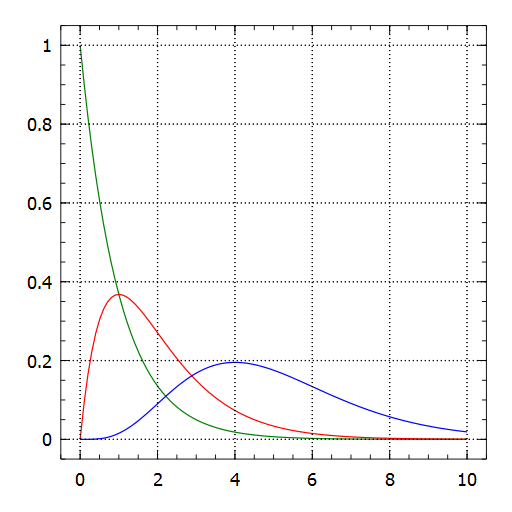
\includegraphics[scale=0.5]{images/gamma_dist_plot.png}
\caption{Page1}
\end{figure}

\subsubsection{\texorpdfstring{Distribution of
\(N_t\)}{Distribution of N\_t}}\label{distribution-of-n_t}

\(N_t\) is defined as the number of arrivals in the intervall $(0,t)$ (see above). By the relation $N_t \geq n \Leftrightarrow T\_n \leq t$, we have

\[ P(N_t \leq n) = P(T_n \leq t) = \int_0^t r^n \frac{u^{n-1}}{(n-1)!}e^{-ru} du \]

This integral can be calculated as (table book)

\[ P(N_t \leq n) = 1 - e^{-rT} \sum_{k=0}^{n-1} \frac{(rT)^k}{k!}\]

Considering integer values for \(n\), we can write
\(P(N_t=n)=P(N_t \geq n)-P(N_t \geq n+1)\). Inserting above expression,
we finally obtain

\[ P(N_t=n) = e^{-rt} \frac{(rt)^n}{n!}\]

which is the Possin distribution with parameter \(rT\). It is
interesting, that it only depends on the product of r and T and not on
the parameters separately. Because it describes a counting process,
\(N_t\) is a discrete random variable.
